%CS-113 S18 HW-3
%Released: 2-March-2018
%Deadline: 16-March-2018 7.00 pm
%Authors: Abdullah Zafar, Waqar Saleem.


\documentclass[addpoints]{exam}

% Header and footer.
\pagestyle{headandfoot}
\runningheadrule
\runningfootrule
\runningheader{CS 113 Discrete Mathematics}{Homework IV}{Spring 2018}
\runningfooter{}{Page \thepage\ of \numpages}{}
\firstpageheader{}{}{}

\boxedpoints
\printanswers
\usepackage[table]{xcolor}
\usepackage{amsfonts,graphicx,amsmath,hyperref,amssymb}
\hypersetup{
    colorlinks=true,
    linkcolor=blue,
    urlcolor=cyan,
}

\title{Habib University\\CS-113 Discrete Mathematics\\Spring 2018\\HW 4}
\author{$hi04031$}  % replace with your ID, e.g. oy02945
\date{Due: 19h, 16th March, 2018}


\begin{document}
\maketitle

\begin{questions}



\question
\begin{parts}
  \part Prove that $1 = -1 \rightarrow 2 = 1$
  
  \begin{solution}
    We can see that Hypothesis in above statement is false, So implication will always be true.
  \end{solution}
  
  \part Let $a,b \in \mathbb{N}$. What's wrong with the following proof:
  \begin{align*}
  a &= b\\
  a^2 &= ab\\
  a^2 - b^2 &= ab - b^2\\
  (a-b)(a+b) &= (a-b)b\\
  a+b &= b\\
  a &= 0
  \end{align*}
  \begin{solution}
    There is a mistake in forth step we know that a=b so a-b will be equals to zero and we can not divide zero by zero. Answer will be 0 = 0 not a = 0!
  \end{solution}

  \part What's wrong with the following proof that shows $2^n = 1, n = \{0,1,2,...\}$, using strong induction on $n$:
  
  \textbf{Base step:} When $n=0, 2^0=1$, so the result holds.
  
  \textbf{Inductive step:} Suppose the result holds for $0\leq n \leq k$. We will show that it holds for $n=k+1$, i.e. that $2^{k+1}=1$.
  
  \begin{align*}
      2^{k+1} &= \frac{2^{2k}}{2^{k-1}}\\
      &= \frac{2^k.2^k}{2^{k-1}}\\
      &= \frac{1.1}{1}\\
      &= 1
  \end{align*}

  \begin{solution}
    There is a mistake in second step and denominator ${2^{k-1}}$  because when we put k = 0. It becomes $2^{-1}$ and that won't be equal to 1 in next step as we can see it in the above proof. 
  \end{solution}
\end{parts}

\question Buckminster Fuller once said: ``None of the world’s problems will have a solution until the world’s individuals become thoroughly self-educated."

The world is full of problems, but which ones should you focus on? According to \href{http://8000hours.org}{80000.org}, the most urgent problems are ``not only \textbf{big}, they're also \textbf{neglected} and \textbf{solvable} - the fewer people working on a problem, the easier it is to make a big contribution. An issue can be big but comparatively well-known and crowded, like climate change, or it can be small but neglected, like land use zoning reform, and therefore also worth considering."

We present a list of the biggest, most solvable and most neglected global issues that would benefit the most from your contribution. You are encouraged to read more about how these problems measure up at \href{https://80000hours.org/articles/cause-selection/}{8000hours.org}.
\begin{center}
\begin{tabular}{ c c c}
Biosecurity & Climate change & Promoting effective altruism\\\\
Institutional decision-making & Risk from AI & Nuclear Security\\\\
Developing world health & Land use reform & Factory farming
\end{tabular}
\end{center}

You are given a set of 9 global challenges - to which you may add one more of your choice - and three order relations on them: \textbf{NB}: ``not bigger than", \textbf{NS}: ``not more solvable than" and \textbf{NN}:``not more neglected than". Using all 10 challenges and your intuition, give unique answers for each of the following. (Well-formatted, syntactically sound answers are encouraged) 

\begin{parts}
\part A poset of width 5
\part A decomposition of size 4
\part A lattice
\part A totally-ordered set
\part A well-ordered set
\end{parts}

(You may refer to the \textbf{Appendix} for a list of definitions)


  \begin{solution}
  \\
    1 = Discrete\\
    2 = Risk from AI\\
    3 = Bio security\\
    4 = Climate change\\
    5 = Nuclear Security\\
    6 = Promotng effective altruism\\
    7 = Institutional decisicion-making\\
    8 = Developing world Health\\
    9 = Factory farming\\
    10 = land use reform\\
    
    $P = \{1,2,3,4,5,6,7,8,9,10\}$\\
     $Q = \{(x,x): x \epsilon S\}$\\
    
    (a)$\{(1,2),(3,4),(5,6),(7,8),(9,10)\} \cup Q\\$ Max Width of Anti-Chain: $\{1,3,5,7,9\}= 5$\\
    \\
    (b)$\{(1,2),(2,3),(1,3),(4,5),(5,6),(4,6),(7,8),(9,10)\} \cup Q$\\
    Family: $\{\{1,2,3\},\{4,5,6\},\{7,8\},\{9,10\}\}$\\
    
    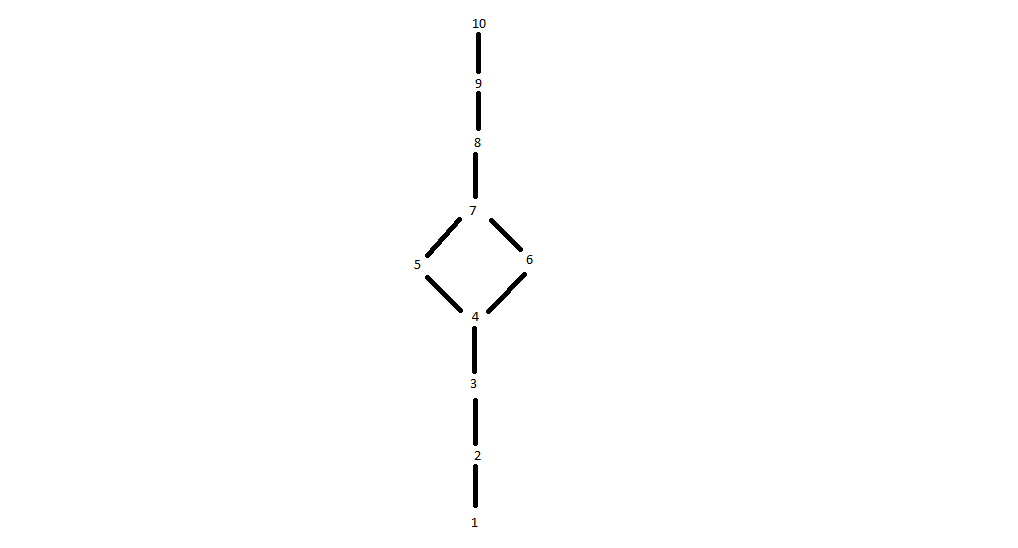
\includegraphics[scale=0.5]{discrete.png}\\
    (c)Above is the Hess diagram representation which represent the lattice (showing the least upper bound and greatest lower bound of every pair)\\
    \\
    (d) We know that a totally order set is a set  in which there is a relation of every element with every other element.Hence every problem will be compareable with other one. Since in part (a) we have already established a poset relation and we can relate each element to every other element according to the grading of solvability Hence it is a totally ordered pair.
     \end{solution}
    (e)We know that it is a totally ordered set in relation of 2 is more solvable than 1 so it will also be a well ordered set. 
 Q  
\question 
A poset $(R, \preccurlyeq)$ is \textbf{well-founded} if there is no infinite decreasing sequence of elements in the poset, i.e. elements $x_1, x_2, \cdots, x_n$ such that $\cdots \prec x_n \prec \cdots  \prec x_2 \prec x_1$. A poset $(R, \preccurlyeq)$ is \textbf{dense} if for all $x \in S$ and $y \in S$ with $x \prec y$, there is an element $z \in R$ such that $x \prec z \prec y$.

Show that the set of strings of lowercase English letters with lexicographic order is neither well-founded nor dense.


  \begin{solution}
  (a) The above statement is not well founded and we can say there is a infinite decreasing sequence $\cdots \prec qqqqr  \prec qqqr \prec qqr  \prec qr \prec r$ which make this set not well founded.\\
 \\
 (b)The set is not dense which can be proven by counter example\\
 Habab and Hababa such that there is no other element that exist between Habab and Hababa\\
  \end{solution}

\question
     Let $S$ and $T$ be two partial orders on a set $A$. Define a new relation $R$ on $A$ by $(x,y)\in R$ iff both $(x,y) \in S$ and $(x,y) \in T$. Prove that $R$ is a partial order on $A$.

    \begin{solution}
    Let the relation be $R = S 
   \cap T$ \\
   In order to prove that R is Partial derivative we need to prove that R is reflexive , anti-symmetric and transitive.\\
   (a) If $(x,x)$ belongs to S and T then $(x,x)$ must exist in R ,so R will be reflexive.\\
   (b) If $(x,y)$ belongs to S and T and $(y,x)$ doesn't belongs to S and T then $(x,y)$ must exist in R while $(y,x)$ doesn't.
    
    (c)All pairs of the form $(x,y)$ and $(y,z)$ in $S$ and $T$ means a pair of form $(x,z)$ will also exist in both.
     
     Since $S \cap T = R$ therefore, for every all pairs of form  $(x,y)$ and $(y,z)$ in $S$ and $T$ will be present in $R$. And for each of the pairs a pair of form $(x,z)$ will also be present making $R$ transitive.
     
      If we don't have the pairs of form $(a, b)$ and $(b,c)$ in any one of relation $S$ or $T$ or $R$, the anti-symmetry will be proved automatically.
      
    As we have proven all the above condition so the relation is partial order 
   \end{solution}

\question Your overly-attached girlfriend / boyfriend has concocted a cruel game to keep you around forever. The game involves piles of excuses - each pile twice as high as the last - of all the times you didn't hang out with them. Stacked in increasing order, the piles look truly endless! 

\begin{figure}[ht]
  \centering
  \includegraphics{excuses.png}
  \caption{That escalated quickly.}
  \label{fig:Piles of excuses}
\end{figure}

The game of \textbf{Gazillion Excuses} is a turn based 2-player game such that at each turn, a player removes a non-zero number of excuses from one of the piles. The player who removes the last excuse wins. Your partner thinks that a sufficiently large number of piles (think gazillion) would keep you playing forever. Little do they suspect that a Discrete Mathematician like yourself has formidable proof skills! Given that you are allowed to go first, \textbf{prove using induction} that you will always win the game of Gazillion Excuses. 

\appendix

\section{Appendix}
Let $\mathcal{P}= (P, \preccurlyeq)$,

\textbf{Chain:} A chain, $C\subseteq P$, is a subset of mutually comparable elements of $P$.\\\\
\textbf{Anti-Chain:} An anti-chain, $A \subseteq P$, is a subset of mutually incomparable elements of $P$.\\\\
\textbf{Width:} The maximum cardinality of an anti-chain of $\mathcal{P}$.\\\\
\textbf{Decomposition:} A decomposition $C$ of $\mathcal{P}$ into chains, is a family $C = \{C_1,C_2,...,C_q\}$ of disjoint chains such that their union is $P$. The size of a decomposition is the number of chains in it.










\end{questions}

\end{document}
